\section{Background}\label{sec:background}

\subsection{MAPF}\label{sec:background_mapf}

The following definitions of Multi-Agent Path Finding (MAPF) follow the ones in~\cite{husvobbass22a}. MAPF is a triple $(V,E,A)$ where \(V,E\) denotes a connected graph, \(V\) being a set of vertices and \(E\) a set of edges connecting them, and \(A\) being a set of agents. For each agent \(a=(s,g) \in A\), \(s \in V\) denotes the starting location and \(g \in V\) denoting the goal location. Every starting position and every goal position are disjoint.
For each discrete time step \(t\in \mathbb{N}_0\), an agent can either, wait at its current vertex or move to a neighbouring one.

The output for MAPF problems is a plan \(\Pi\). A plan is a collection $(\pi_a)_{a\in A}$ of finite sequences in $(V,E)$ where each sequence $\pi_a$ is represented by a finite sequence of adjacent or identical vertices in $V$ from $s$ to $g$ for agent $a = (s,g)$. We use \(\pi_a (t) = v\) to denote that agent \(a\) is located at vertex \(v\) at time step \(t\). 
For each \(a=(s,g) \in A\), we have $\pi_a(0) = s$ and  $\pi_a(|\pi_a|-1) = g$, where $|\pi_a|$ gives the length of sequence $\pi_a$. Generally, for any \(a=(s,g)\) and any $0 \leq t \leq |\pi_a|-1$, we have \(\pi_a(t) \in V\). In addition, we also have $(\pi_a(t),\pi_a(t+1))\in E$ with $0 \leq t < |\pi_a|-1$

A plan is considered  \textit{valid} if, taken pair wisely, sequences are collision-free. A vertex conflict occurs whenever two different agents occupy the same vertex at the same time step. Formally, we have \(conflict(a,a',t)\) if given any $a,a'\in A$  and $t\in\mathbb{N}_0$, we have $\pi_a(t) = \pi_{a'}(t)$. An edge conflict (or swapping conflict) occurs whenever two agents exchange their position or are using the same vertex at the same time. We have \(conflict(a,a',t)\) if given any $a,a'\in in A$  and $t\in\mathbb{N}_0$, we have $\pi_a(t-1) = \pi_{a'}(t)$ and $\pi_a(t) = \pi_{a'}(t-1)$.

A plan $(\pi_a)_{a\in A}$ has a conflict, if a conflict $(a, a',t)$ occurs in $(\pi_a)_{a\in A}$ for some pair $a,a'\in A$ of agents and a time step $t\in\mathbb{N}_0$.

\textit{Sum-of-costs} and \textit{makespan} of a plan $(\pi_a)_{a\in A}$ are respectively defined as such; $\sum_{a\in A} (|\pi_a| - 1)$ and $\max_{a\in A} (|\pi_a| - 1)$.

Furthermore, we assume that graphs have Cartesian coordinate system, which means we can represent them as a grid. 

\subsection{ASP}

Answer Set Programming~\cite{ankolisc05a} (ASP)is an approach for declarative logic programming. In a nutshell, programmer aims to describe problems instead of solving them.

A logic program \(P\) is defined by a finite set of rules. Given a set of atoms \(\mathcal{A}\), a rule \(r\) is of the form 
\[
    a_0 \leftarrow a_1, \dots, a_n,not~a_{n+1}, \dots,not~a_m     
\] 
with \(a_i \in \mathcal{A}, 0 \leq i \leq m\). An atom preceded by \(not\) refer to its \textit{default negation}. We call literal an atom or its default negation.

In a rule \(r\), \(a_0\) represents the head of the rule and \(\{a_1, \dots, a_m,not~a_{m+1}, \dots,not~a_n\}\) the body of the rule. We will refer respectively to them as such; \(H(r)\) the head of the rule and \(B(r)\) the body of the rule. We define \(B(r) = B^+(r) \cup B^-(r) \) and \(B(P) = \{B(r) |r \in P\}\). For each rule \(r\) in \(P\), \(B^+(r) =\{ a_0 \leftarrow a_1, \dots, ~a_n\}\), \(B^-(r) =\{ a_{n+1}, \dots, ~a_m \}\) and \(H(r) = a_0\). 
A \textbf{fact} is defined as a rule with an empty body. On the other hand, with an empty head, the rule becomes an integrity \textbf{constraint}.
We define \(P_X\) as the reduct of a program \(P\) relative to a set of assigned atom \(X\).
\[
    P_X = \{H(r) \leftarrow B^+(r) | r \in P, X \cap B^-(r) = \emptyset\}
\]

A set \(X\) of atoms is a stable model of \(P\) if \(P_X\) is the smallest set under \(P_X\).



For instance, lets encode the following problem. We want to pack as many object in our bag respecting the maximum authorized weight. First lets denote the possible objects.

\begin{minipage}[H]{\linewidth}
\begin{lstlisting}[style=mystyle]
object(trousers, 3).
object(tshirt, 2).
object(toothbrush, 1).
object(camera, 2).
object(tent, 8).
object(drinks, 2).
object(sandwiches, 2).
object(laptop, 3).
object(tablet, 2).
\end{lstlisting}
\end{minipage}


To decide which objects to pick, we utilize a choice rule. A choice rule provide a choice over a set of atoms.

\begin{minipage}[H]{\linewidth}
\begin{lstlisting}[style=mystyle]
    {pick(N,W):object(N,W)}.
\end{lstlisting}
\end{minipage}

Here, the choice rule allows for various combinations of objects to be picked. We then enforce a constraint that ensures the total weight of the selected objects does not exceed 20. This constraint is expressed using an aggregate function within an integrity constraint:

\begin{minipage}[H]{\linewidth}
\begin{lstlisting}[style=mystyle]
    :- #sum{W : pick(N,W)} > 20. 
\end{lstlisting}
\end{minipage}

In addition, we add some normal rules and constraint to enforce \textit{picking} some items if some other items are picked. The first two constraint implies that, if the \textit{tent} object is picked, then it is not possible that \textit{drinks} and \textit{sandwiches} objects are not picked. The two last normal rules implies that, if \textit{laptop} and \textit{tablet} are picked, a \textit{charger} item is added to the pool of object and is picked.

\begin{minipage}[H]{\linewidth}
    \begin{lstlisting}[style=mystyle]
    :- pick(tent), not pick(drinks).
    :- pick(tent), not pick(sandwiches).
    
    object(charger,1) :- pick(laptop,W1), pick(tablet,W2).
    pick(charger,W) :- object(charger,W). 
\end{lstlisting}
\end{minipage}


Lastly, we want to maximize the weight of the bag while still keeping it under 20. To achieve this, we use an optimization statement that seeks to find the maximum weight among the available combinations:

\begin{minipage}[H]{\linewidth}
\begin{lstlisting}[style=mystyle]
    #maximize{W : pick(N,W)}. 
\end{lstlisting}
\end{minipage}
This encoding will yield the optimal combination of objects to pack into the bag, maximizing the weight without having the weight above 20.

\subsection{Solving MAPF with ASP}

\subsubsection{Instance Format}

A MAPF instance is defined using the following predicates

\begin{enumerate}
    \label{list:instance_format_explanation_part1}
    \item \(vertex/1\) which describe a vertex of the graph with a tuple \((X,Y), X,Y \in \mathbb{N}^+\) expressing the position.
    \item \(edge/2\) which describe an edge between two vertices. With two tuple \((X,Y), X,Y \in \mathbb{N}^+\) expressing the endpoints of the edge.
    \item \(agent/1\) which define agents of an instance with its identifier as parameter
    \item \(start/2\) which describe the starting position of an agent. With an agent identifier as first parameter and a vertex as second parameter expressing the starting position.
    \item \(goal/2\) which describe the goal position of an agent. With an agent identifier as first parameter and a vertex as second parameter expressing the goal position. 
\end{enumerate}

We introduce optional predicates used for the computation of individual paths. They are defined as such:

\begin{enumerate}
    \label{list:instance_format_explanation_part2}
    \item \(shortestpath\_length/2\)  represents the length of the shortest path of an agent. With the identifier of an agent as first parameter and the length of a shortest path for the associated agent.
    \item \(makespan/1\)  describes the maximum makespan of the instance. It can also be defined as a \(horizon\) constant
\end{enumerate}

For example, the following facts describe the graph illustrated by figure~\ref{lst:instance_format_example}.

\begin{minipage}[H]{\linewidth}
\begin{lstlisting}[style=mystyle, caption={Example of instance format}, label={lst:instance_format_example}]
agent(1). start(1,(2,1)). goal(1,(2,4)).
agent(2). start(2,(2,3)). goal(2,(2,5)).
agent(3). start(3,(5,4)). goal(3,(1,4)).

vertex((2,3)). vertex((1,4)). vertex((2,4)).
vertex((3,4)). vertex((4,4)). vertex((2,1)).
vertex((5,4)). vertex((2,5)). vertex((2,2)).

edge((2,4),(1,4)). edge((3,4),(2,4)).
edge((4,4),(3,4)). edge((5,4),(4,4)).
edge((2,3),(2,2)). edge((2,4),(2,3)).
edge((2,5),(2,4)). edge((2,2),(2,1)).
edge((2,3),(2,4)). edge((2,4),(2,5)).
edge((2,1),(2,2)). edge((2,2),(2,3)).
edge((1,4),(2,4)). edge((2,4),(3,4)).
edge((3,4),(4,4)). edge((4,4),(5,4)).

% Optional 
shortestpath_length(1,3).
shortestpath_length(2,2).
shortestpath_length(3,4).

makespan(4).
\end{lstlisting}
\end{minipage}


\begin{figure}[H]
    \centering
    \caption{Illustrated graph of the instance format example~\ref{lst:instance_format_example}}\label{fig:illustrated_instance_format_example}
    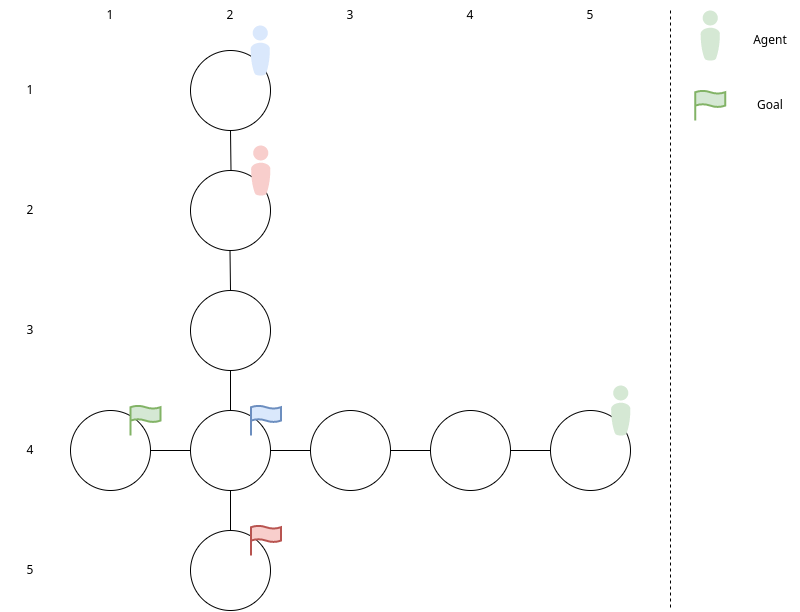
\includegraphics[width=\widthimg]{img/illustrated_instance_format_example.drawio.png}
\end{figure}


\subsubsection{Encoding}

As baseline for ASP MAPF solver, we adapt an encoding available in  \textit{asprilo}~\cite{geobotscsangso18a}, which we call \textbf{base MAPF encoding}. In the encoding, we use two primary predicates:

\begin{enumerate}\label{list:base_mapf_encoding_predicate_explanation}
    \item \(at(R,P,T)\)  represents the position \(P\) of an agent \(R\) at time step \(T\).
    \item \(move(R,U,V,T)\) represents the movement from vertex \(U\) to vertex \(V\) at time step \(T\).
\end{enumerate}

\begin{minipage}[H]{\linewidth}
\begin{lstlisting}[style=mystyle, caption={Base MAPF encoding}, label={lst:base_mapf_encoding}]
    at(R,P,0) :- start(R,P). |\label{line:init_at}|
    time(1..horizon). |\label{line:init_horizon}|

    {move(R,U,V,T) : edge(U,V)} 1 :- agent(R), time(T). |\label{line:generating_moves}|

    at(R,V,T) :- move(R,_,V,T). |\label{line:generating_at}|
    :- move(R,U,_,T), not at(R,U,T-1). |\label{line:constraining_moves}|
    at(R,V,T) :- |\label{line:waits}|
        at(R,V,T-1), 
        not move(R,V,_,T), 
        time(T). 

    :- { at(R,V,T) }!=1 , agent(R), time(T). |\label{line:one_at_per_t}|

    :- {at(R,V,T) : agent(R)} > 1, vertex(V), time(T). |\label{line:vertex_conflict}|
    :- move(_,U,V,T), move(_,V,U,T), U < V. |\label{line:edge_conflict}|
        
    :- goal(R,V), not at(R,V,horizon). |\label{line:goal_reached}|
\end{lstlisting}
\end{minipage}

In the initial section of encoding~\ref{lst:base_mapf_encoding}, we define, respectively on lines~\ref{line:init_at} and~\ref{line:init_horizon}, the starting positions of each agent and their allocated time using the constant \textit{horizon}.


The rule at line~\ref{line:generating_moves} describes how movements are performed. A possible interpretation could be; for each agent at each available time step and among all available edge going from \(U\) to \(V\), we pick at most one to define one movement at each time.

The rule at line~\ref{line:generating_at} states that if a move action is performed by the agent from any location (indicated by \textunderscore) to a different one, the agent is positioned at this destination at this time step.
Then, the rule at line \ref{line:constraining_moves} is a constraint that ensures consistency and coherence in the agent's locations over time. It prevents agents from moving towards a location without having been to the source location of the move at the previous time step. 
Furthermore, the rule at line~\ref{line:waits} specifies that if an agent does not make a move at a specific time step, their location remains the same. 
Rule \ref{line:one_at_per_t} ensures that an agent was at most one position at a time.

Line~\ref{line:vertex_conflict} outline vertex collision with a constraint rules;  for each vertex, at most one agent can be positioned at a vertex.
Secondly, the rule~\ref{line:edge_conflict} ensure that, no movement from vertex \(U\) to \(V\) and no movement from \(V\) to \(U\) are issued at the same time.
Lastly, the rules~\ref{line:goal_reached} forces that an agent is at their goal at the last timepoint.

The output of the encoding is the predicate \(at/3\). 
